%!TEX root = ../main.tex
Strictly proper scoring rules and associated Bregman divergences determine an \emph{information geometry} of probability distributions. In this section I aim to develop an understanding of the differences between various scoring rules and by visualising these geometric structures each of them give rise to.

The central object of interest in information geometry is the smooth Riemannian manifold of probability distributions that the divergence function induces, called the \emph{statistical manifold}. In this section, our goal is to create low-dimensional maps of these statistical manifolds in such a way that distances measured between points on the map correspond to geodesic distances measured on the manifold as precisely as possible. In particular, we will focus on one and two-dimensional maps of families of distributions parametrised by at most two continuous parameters.

First, it is important to note that a perfect embedding of this sort does not always exist. As an illustration, think of the well-known practical problem of creating a two-dimensional map of the surface of the Earth. The surface of Earth is approximately a sphere, which is a smooth two-dimensional Riemannian manifold, just as the statistical manifolds we would like to map in this chapter. The sphere can be parametrised by two parameters, longitude and latitude. Still, it is impossible to stretch this surface out and represent it faithfully in two dimensional Cartesian coordinate system. This problem -- representing the surface of a three-dimensional object as part of a two-dimensional plane -- is in fact at the core of cartography, and is called \emph{map projection}. When drawing a full map of the surface of the Earth, usually the manifold has to be cut up at certain places, but even then, the embedding is only approximate, and distances are only correct locally. This is why on Google maps Finland appears about twice as large as France, even though in reality it is only about half the size of France. There are various map projections used in cartography, and the purpose for which the map is used dictates what kind of distortions are tolerable, and what is not.

Having understood that a perfect map of two-dimensional statistical manifolds cannot necessarily be produced, I will resort to approximate embedding techniques developeded in the machine learning community. These approximate embedding procedures numerically find a low-dimensional map that best represents distances on the statistical manifold defined by a particular scoring rule and divergence, optimising an appropriately defined objective function. In this chapter I will employ an algorithm analogous to the ISOMAP algorithm \citep{isomap}, originally developed for dimensionality reduction and visualisation of high-dimensional data.

This chapter is organised as follows. I will first review crucial mathematical concepts in information geometry. Then I will introduce a general algorithm for numerically mapping out Riemannian manifolds induced by strictly proper scoring rules. Finally, I show maps of one- and two-parameter exponential families of distributions with respect to various divergence metrics introduced in chapter \ref{sec:scoring_rules}.

\section{Information geometry}

Strictly proper scoring rules and their associated divergence functions induce a geometry over probability distributions, that we will call the information geometry. Under suitable smoothness assumptions, probability distributions form a smooth Riemannian manifold \citep{Amari,Dawid}, on which the squared local distance is

\begin{equation}
	ds^2(P) = \frac{1}{2} \scalar{P}{\ddot{H}(P)P},
\end{equation}
Where $\ddot{H(P)}$ is the Hamiltonian of the entropy function $H(P) = \mathbb{H}_{\score}$ at $P$. For discrete distributions, when $\Xe={1,2,\ldots}$, denoting $p_i\defeq P[X=i]$ we can write this squared distance as

\begin{equation}
	ds^2 = \frac{1}{2} \sum_{i,j} \frac{\partial^2 H}{\partial p_i\partial p_j} dp_{i} dp_{j}.
\end{equation}

The local distance between distributions is therefore controlled by the curvature of the entropy function: the higher the curvature, the more amplified the distances are locally. The following Taylor expansion shows how this local distance is related to the Bregman divergences defined by the entropy function:

\begin{statement}[Taylor expansion of Bregman divergences]
	Let $H:\Theta\mapsto\Reals$ be a smooth, strictly concave function and $\divergence{H}{\cdot}{\cdot}$ the Bregman divergence it induces. For infinitesimally small $dP\in\Theta$ the following approximation holds:
	\begin{equation}
		\divergence{H}{P}{P+ dP} \approx \frac{1}{2} \sum_{i,j} \frac{\partial^2 \mathbb{H}_{\score}}{\partial p_i\partial p_j} dp_{i} dp_{j} \approx   \divergence{H}{P + dP}{P}
	\end{equation}
	\begin{proof}
		We prove the left-hand equation first:
		\begin{align}
			\frac{\partial}{\partial q_i} \divergence{H}{P}{Q} &=  -\frac{\partial}{\partial q_i} H(Q) +    \frac{\partial}{\partial q_i}\scalar{\nabla_{Q} H(Q)}{Q-P}\\
				&=  - \frac{\partial}{\partial q_i} H(Q) +  \frac{\partial}{\partial q_i}\sum_{j} \frac{\partial}{\partial q_j} H(Q) (q_j - p_j)\\
				&= - \frac{\partial}{\partial q_i} H(Q)  + \frac{\partial}{\partial q_i} H(Q) + \sum_{j} \frac{\partial^2}{\partial q_i \partial q_j} H(Q) (q_j - p_j)\\
				&= \sum_{j} \frac{\partial^2}{\partial q_i \partial q_j} H(Q) (q_j - p_j)
		\end{align}
		hence by first order Taylor expansion around $P$:
		\begin{align}
			\divergence{H}{P}{P+dP} &\approx  \divergence{H}{P}{P+dP}+ \frac{1}{2}\scalar{dP}{\left.\nabla_{Q}\divergence{H}{P}{Q}\right\rvert_{Q=P}}\\
				&= \frac{1}{2} \sum_{i} dp_i \sum_{j} \frac{\partial^2 H(P)}{\partial p_i\partial p_j} dp_j \\
				&= \frac{1}{2} \sum_{i,j} \frac{\partial^2 H(P)}{\partial p_i\partial p_j} dp_{i} dp_j
		\end{align}
		
		Similarly in the other direction
			\begin{align}
					\frac{\partial}{\partial q_i} \divergence{H}{Q}{P} &=  \frac{\partial}{\partial q_i} H(Q) +     \frac{\partial}{\partial q_i}\scalar{\nabla_{P} H(P)}{P - Q}\\
						&=  \frac{\partial}{\partial q_i} H(Q) + \frac{\partial}{\partial q_i}\sum_{j} \frac{\partial}{\partial p_j} H(P) (p_j - q_j)\\
						&=  \frac{\partial}{\partial q_i} H(Q)  - \frac{\partial}{\partial p_i} H(P)\\
						&= \dot{H}(Q) - \dot{H}(P)
			\end{align}
			Note that for small deviation $dP$, the derivative can be written as
			\begin{align}
				\frac{\partial}{\partial dP} \divergence{H}{P+dP}{P} = \dot{H}(P+dP) - \dot{H}(P) \approx  \ddot{H}(P) dP
			\end{align}
			therefore, via Taylor expansion we get that for small $dP$
			\begin{align}
				\divergence{H}{P}{P+dP} &\approx \frac{1}{2} \scalar{dP}{\ddot{H}(P)dP}\\
					&= \frac{1}{2} \sum_{i,j} \frac{\partial^2 H(P)}{\partial p_i\partial p_j} dp_{i} dp_j
			\end{align}
	\end{proof}
\end{statement}

Hence, the distance on the manifold can be approximated locally as half the squareroot of the divergence function. Even though a Bregman divergence function is generally asymmetric, for infinitesimally small differences it becomes symmetric, and therefore it does not matter which direction we use if we want to approximate local distances on the manifold. Below we will use the following local approximation:

\begin{corollary}[Local approximation to geodesic distance]
	The geodesic distance between distributions $P$ and $Q$ on the statistical manifold defined by the scoring rule $S$ can be approximated as follows.
	\begin{equation}
		\mbox{distance}(P,Q) \approx \sqrt{\divergence{S}{P}{Q} + \divergence{S}{Q}{P}} \label{eqn:local_approximation}
	\end{equation}
\end{corollary}

Another core concept in information geometry is that of geodesics and geodesic distances between distributions:

\begin{definition}[Riemannian geodesic]
	Let $P_1$ and $P_2$ be two probability distributions and $d_H$ a Bregman divergence. Let $\mathcal{P}=\{P(t),t\in[0,1]\}$ a smooth, differentiable path on the manifold such that $P(0)=P_1$ and $P(1)=P_2$. The length of the curve $\mathcal{P}$ is defined as
	\begin{equation}
		l(\mathcal{P}) = \int_{0}^{1} \sqrt{ \scalar{\dot{P}(t)}{\ddot{H}(P(t))\dot{P}(t)}} dt \label{eqn:Riemannian_length}
	\end{equation}
	A Riemannian geodesic between $P_1$ and $P_2$ is a path, whose length is minimal. The length of such a path is called the geodesic distance between $P_1$ and $P_2$.
\end{definition}


\section{Approximate embedding of Riemannian manifolds}

Our goal in the rest of this chapter is going to be to create maps of statistical manifolds, such that the Euclidean distances between distributions on the maps approximate geodesic distances on the manifold as faithfully as possible. However, geodesic distances on general, non-trivial Riemannian manifolds are hard to compute analytically. There are two main technical difficulties that arise:

\begin{enumerate}
	\item The integral defining the Riemannian length of a given path (eqn.\ \eqref{eqn:Riemannian_length}) can be hard to compute analytically, even if an analytical expression for the local squared distance $ds^2$ exists.
	\item The geodesic distance between $P$ and $Q$ is the minimum of the length of any path that connects $P$ and $Q$. This minimisation over all paths is a non-trivial one and is very hard to carry out exactly, even if an analytical expression for the length existed.
\end{enumerate}

Therefore, if we want to create maps of arbitrarily complex statistical manifolds, we will have to resort to numerical approximations to geodesic distances. To sidestep both computational problems at once, we are going to restrict geodesic paths between distributions $P$ and $Q$, to paths on a graph of neighbouring points on the manifold.

Consider a graph, whose vertices are points on the manifold and we draw an edge between pairs of points that are close enough to each other. We will refer to this as a local neighbourhood graph. As neighbours in this graph are assumed to be close, the geodesic distance between neighbours is approximately the same as the local squared distance, and can be approximated using Eqn.\ \ref{eqn:local_approximation}. Let us define this approximate distance between neighbours as the weight of the edge between them. The length of any path that travels trough a series of vertices of the neighbourhood graph can then be approximated as the sum of edge weights between subsequent points the path travels trough. It is easy to see that if the vertices of this neighbourhood graph cover the manifold densely enough, path lengths on this graph can be used to approximate the length of any smooth path on the manifold. Computing geodesic distances then amounts to finding the shortest path on the neighbourhood graph, for which polynomial time algorithms exist.

This idea of using shortest paths in a local neighbourhood graph as approximation to geodesic distances has been used in the context of manifold learning and forms the basis of the ISOMAP algorithm \citep{isomap}. In ISOMAP, a set of points that are assumed to conform to a manifold are given to us as the input to the algorithm, and we have to recover the latent geometric structure. In this section, we are free to chose a set of distributions that will constitute the vertices of the neighbourhood graph. In most cases as we will visualise manifolds of parametric classes of distributions it is practical to choose a uniformly or logarithmically spaced grid in parameter space, where the neighbourhood structure is naturally defined by the grid itself.

We will follow the following procedure to produce a map of the statistical manifolds induced by scoring rules.

\begin{enumerate}
\item take a set of probability distributions, preferably such that they relatively densely cover an interesting region on the manifold. In most cases we will choose a square grid in an appropriately chosen parameter-space.
\item compute approximate geodesics:
\begin{enumerate}
	\item construct a graph over the sampled distributions as nodes, such that we draw edges between each distribution and its $k$ nearest neighbours. The weight of each edge is the squareroot of the symmetrised divergence between the two distributions, as in Eqn.\ \eqref{eqn:local_approximation}.
	\item compute the shortest path on the resulting graph between every pair of points on the graph
\end{enumerate}
\item use metric multidimensional scaling with the approximate geodesic distance matrix as input to embed the set of distributions as points a low-dimensional Euclidean space.
\end{enumerate}

\subsection{Bernoulli distributions}

Let us first look at the simple and special case of one dimensional statistical manifolds of Bernoulli distributions. Bernoulli random variables, often referred to as biased coin-flips, have a binary outcome: positive with probability $p$ and negative with probability $1-p$. The probability $p$ is a real valued parameter, hence Bernoulli distributions conform to a one-dimensional manifold.

One dimensional Riemannian manifolds are special, as these are always homeomorphic to either the real line $\Reals$, or the circle. In addition, one dimensional statistical manifolds induced by strictly proper scoring rules are always homeomorphic to the real line, never to a circle. So the only difference between various statistical manifolds is how the real line is stretched and compressed at various locations.

In Figure \ref{fig:Bernoulli_manifold} I illustrate the differences between the statistical manifolds induced by the logarithmic, Brier and spherical scoring rules using the numerical embedding technique outlined above. As KL divergence between $p$ and $q$ is not bounded and diverges for $q\rightarrow 0$ and $q\rightarrow 1$, the statistical manifold corresponding to this divergence will span the whole extended real line $[-\infty,\infty]$. The Brier and spherical divergences are bounded, hence the manifold becomes an finite interval of $\Reals$.

To visualise the differences between these manifolds, I started with a linearly spaced grid of $33$ parameter values in the interval $[0+\epsilon,1-\epsilon]$, with $\epsilon = 10^{-3}$. In this interval of parameter values all three divergences are bounded, so when applying the ISOMAP procedure, this part of the manifold gets mapped to a finite segment in each of the three cases. As scoring rules - and divergences - are equivalent up to a multiplicative constant, we can scale the resulting intervals arbitrarily to be of the same length. Figure \ref{fig:Bernoulli_manifold} shows the resulting manifold structure for the three divergences. As the Brier divergence between $p$ and $q$ is the squared Euclidean distance between $p$ and $q$, the geodesic distance on this statistical manifold is simply the Euclidean distance. Therefore, as expected, the uniformly spaced grid of probabilities is represented as a uniformly spaced grid of points on this map of the manifold.

As we can see, compared to the Brier score, the KL divergence is more sensitive to differences in very small (close to 0) and large (close to 1) probabilities, but puts less emphasis on discriminating between intermediate values close to $p=0.5$. Remember that the statistical manifold corresponding to the KL divergence extends to $-\infty$ and $\infty$ and in Figure \ref{fig:Bernoulli_manifold} we only show a segment from it.

When using the KL divergence or the log-score in practical situations, such as to train binary classifiers, we should therefore expect that much of the statistical power is going to be spent on faithfully representing small probabilities, as this is where the resolution of the divergence is highest. This behaviour is not always desirable: Imagine we were to model the probability that users click on certain news articles on an on-line news website. In this application, most potential clicks have negligible probability, but some user-article combinations may have probabilities closer to $0.5$. If we are to build a recommender system based on this analysis, it is modelling these large probabilities that will be of importance. In this case we are better off using the Brier-score, rather than the log-score which would spend most effort on modelling how small the small probabilities are exactly.

\begin{figure}
	\begin{center}
	 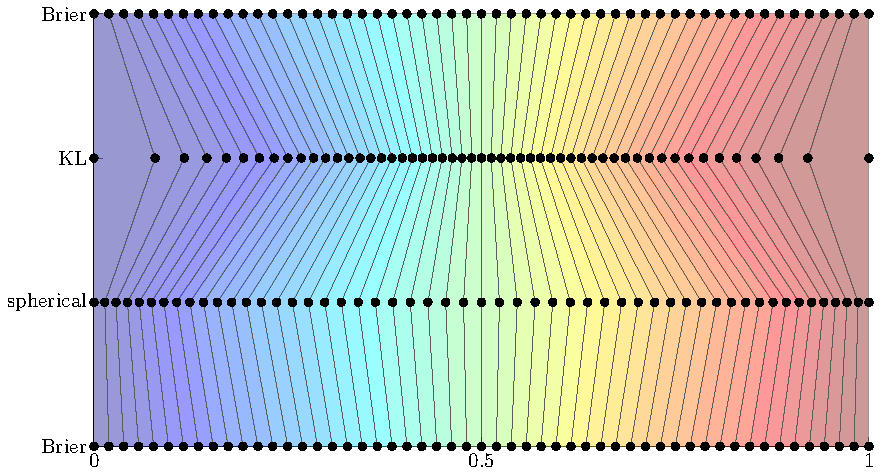
\includegraphics{/Users/fhuszar/Dropbox/thesis/matlab/manifold/figs/Bernoulli_comparison.pdf}
	\end{center}
	\caption{Illustration of the differences between the Brier, spherical, and KL divergences between single parameter Bernoulli distributions. Each horizontal line of dots shows the embedding Bernoulli distributions corresponding to an uniform grid of parameter values between $0+\epsilon$ and $1-\epsilon$ on the statistical manifold induced by (from top to bottom) the Brier, KL, spherical and again the Brier score.  Dots representing the same distributions on the different manifolds are connected. This, together with colouring, highlights the differences between the manifolds.
	The Brier divergence is equivalent to the squared Euclidean distance between parameter values, therefore when mapped by Brier divergence, parameters are evenly spaced along the line segment\emph{(top, bottom)}. The KL divergence places emphasis on discriminating between  small probabilities, therefore the manifold is stretched out as the parameter approaches $0$ and $1$. In fact the KL divergence is not bounded, and the full manifold of Bernoulli distributions stretches to the entire real line. By contrast, the spherical score focuses more on probability values around $0.5$.}
	\label{fig:Bernoulli_manifold}
\end{figure}

\begin{figure}
	\begin{center}
	 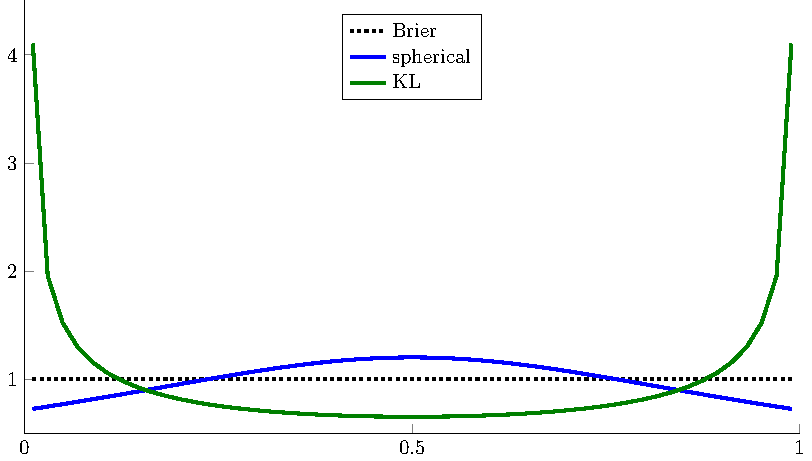
\includegraphics{/Users/fhuszar/Dropbox/thesis/matlab/manifold/figs/Bernoulli_magnification.pdf}
	\end{center}
	\caption{Illustration of the differences between local distances on statistical manifolds of Bernoulli distributions. Each line shows the magnitude of the local distance on the manifold relative to the Euclidean distance as a function of the parameter value. Distance on the Brier manifold is equivalent to the Euclidean distance, hence it's relative magnitude is constant \ref{}. The KL divergence gives rise to increasing local distances as the parameter approaches $0$ and $1$ \ref{}. The spherical score induces a local distance that is largest at $0.5$ \ref{}.}
	\label{fig:Bernoulli_squareddistance}
\end{figure}

Figure \ref{fig:Bernoulli_manifold} also shows the statistical manifold induced by the spherical score. As we can see, relative to the Brier score, the spherical score has a larger resolution among intermediate probabilities close to $0.5$ than around small probabilities closer to $0$ and $1$. Therefore in applications where modelling probabilities closer to $0.5$ is important, the spherical score may be an even more appropriate choice than the Brier score.

In Figure \ref{fig:Bernoulli_squareddistance} I plotted the local distance $\sqrt{\ddot{\mathbb{H}}_{\score}[p]}$ as a function of $p$ for the three different scores illustrated in Figure \ref{fig:Bernoulli_comparison}. Higher value of this curve means that the scoring rule has a ``higher resolution'' locally. It is another visualisation that allows us to observe that relative to the Brier score, the logarithmic score focuses more on probabilities close to $0$ and $1$, whilst the spherical divergence focuses more on probabilities close to $0.5$.

% We note that in this simple example of binary random variables, a map of the manifold could have been drawn exactly, without the need for the numerical approximations used by the ISOMAP technique. It is easy to see that given a scoring rule $\score$ transforming the real line by the gradient of the entropy function $\dot{\mathbb{H}}_{\score}$ yields an embedding that faithfully represents the statistical manifold induced by $\score$. For example, the geodesic distance on the Brier manifold is simply the Euclidean distance, and indeed the gradient of the entropy function is essentially the identity $\dot{\mathbb{H}}_{Brier}[p] = -p$. The gradient of the Shannon's entropy diverges to infinity $p\rightarrow 0$ and to negative infinity as $p\rightarrow 1$, which shows that this statistical manifold spans the entire real line.

% The fact that we can compute an exact embedding allows us to evaluate how well our ISOMAP-based numerical technique works. As the embedding is unique only up to translation and reflection, we \TODO{do this numerically, maybe}.

\subsection{Gaussian distributions}

Gaussian distributions are probably the most important family of distributions due to their convenient analytical properties. They are often used in density estimation, regression, approximate inference and more advanced non-parametric models such as Gaussian process regression.

The KL divergence between two univariate Gaussian distributions is available in a closed form and is given by the following formula:

\begin{equation}
	\KL{\Normal_{\mu_1,\sigma_1}}{\Normal_{\mu_2,\sigma_2}} = \frac{\left(\mu_1 - \mu_2\right)^2}{2\sigma_2^2} + \frac{1}{2}\left(\frac{\sigma_1^2}{\sigma_2^2} - 1 - \log\frac{\sigma_1^2}{\sigma_2^2}\right)
\end{equation}

In this case as Gaussian distributions have two parameters, the distributions are going to conform to a two dimensional statistical manifold, as illustrated in Figure \ref{fig:normals_manifold}. We used the ISOMAP technique on a linearly spaced grid of parameters to produce this approximate embedding. We can observe that assuming that $P$ and $Q$ have the same mean, the larger their variance, the easier it becomes to distinguish between them. Otherwise the manifold structure is symmetrical.

\begin{figure} % Normals 2D embedding KL
	\begin{center}
	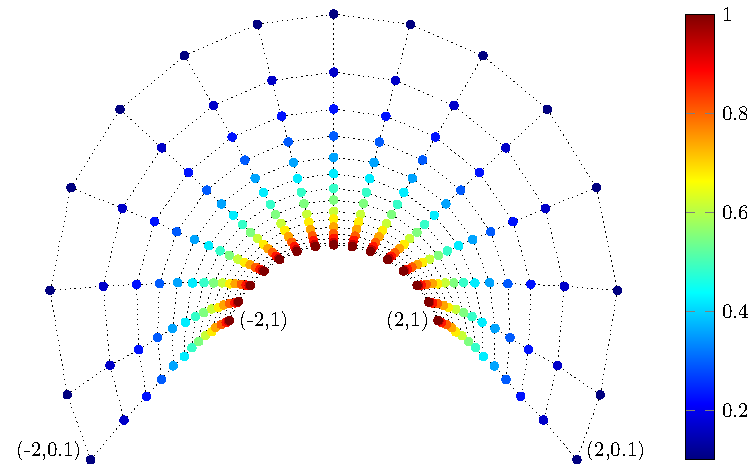
\includegraphics{/Users/fhuszar/Dropbox/thesis/matlab/manifold/figs/Normal_meanvar.pdf}
	\end{center}
	\caption{Map of Normal distributions on the statistical manifold induced by the logarithmic score and KL divergence. Distributions are chosen from a uniform grid in parameter space, with mean ranging between $-2$ and $2$ \emph{(left to right)}, and standard deviation between $0.1$ and $1$ \emph{(from outside inwards)}. The labels show distributions at the corners of this grid.  Dots of the same colour show distributions with the same standard deviation. It can be clearly seen that distributions with lower standard deviation are spread out more than those with a higher standard deviation, giving rise to a characteristic fan-like structure.}
	\label{fig:Normal_meanvar}
\end{figure}

\begin{figure} % zero-mean Normals KL, kernel, Brier comparison plot
	\begin{center}
		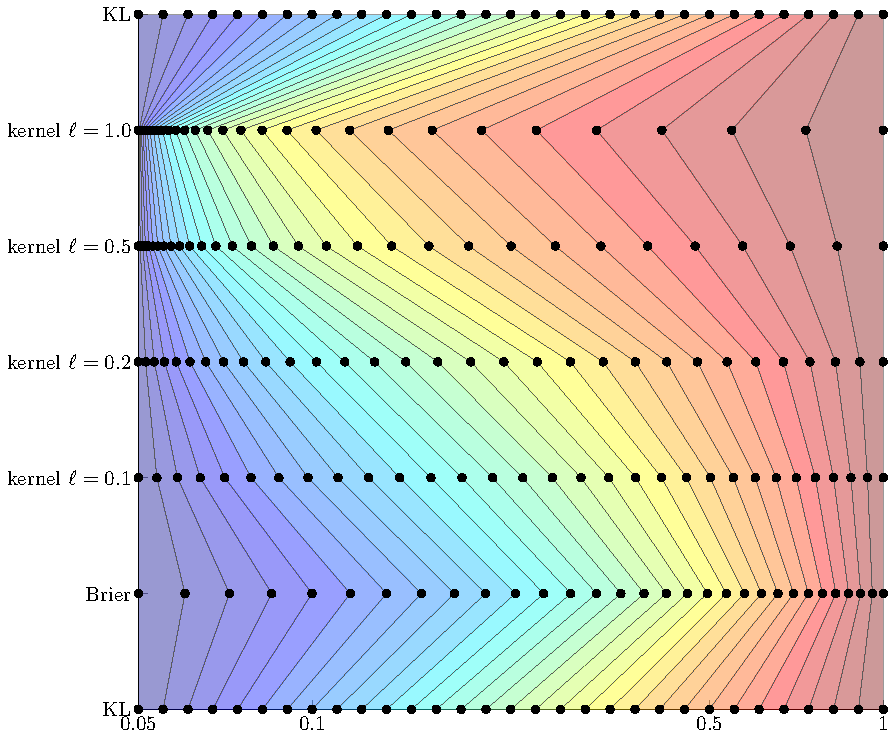
\includegraphics{/Users/fhuszar/Dropbox/thesis/matlab/manifold/figs/Normal_varonly_comparison.pdf}
	\end{center}
	\caption{ Illustration of the differences between the statistical manifolds of Normal distributions induced by the KL, Brier and kernel divergences. Each horizontal line of points shows the one-dimensional manifold of zero-mean Gaussians. The dots correspond to distributions with logarithmically spaced variance between $\sigma_{min}=0.05$ and $\sigma_{max}=1$. When mapped according to the KL divergence, these distributions become evenly spaced \emph{(top,bottom)}. Compared to the KL, the Brier score \emph{(second from bottom)} places more emphasis on disriminating between narrower distributions. In this range $0.05 \leq \sigma \leq 1$ the kernel divergence with bandwidth $\ell=0.1$ \emph{(third from bottom)} approximately mimics the behaviour of the KL divergence. As we use the kernel score with increasing brandwith \emph{(from bottom to top)}, we can see that the focus shifts from narrow distributions towards distributions with larger variance.}
	\label{fig:Normal_varonly_comparison}
\end{figure}

\begin{figure} % zero-mean Normals relative local distance plots
	\begin{center}
	  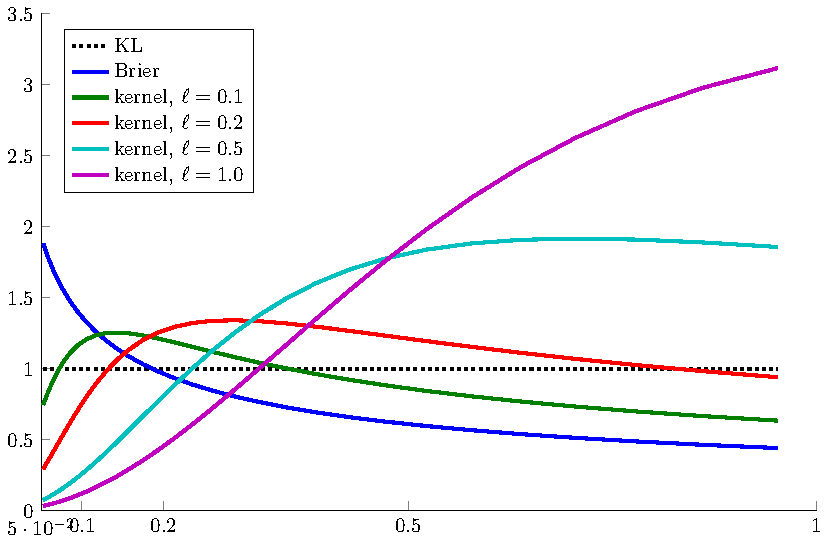
\includegraphics{/Users/fhuszar/Dropbox/thesis/matlab/manifold/figs/Normal_varonly_magnification.pdf}
	\end{center}
	\caption{Illustration of the differences between local distances induced by various scoring rules on the statistical manifold of zero-mean Normal distributions. Each line shows the magnitude of the local distance on each manifold relative to that induced by the KL divergence as a function of variance. Relative to the KL, the kernel divergence induces distances that are magnified around a region depending on the bandwidth of the kernel. As the bandwidth increases, this magnified region shifts towards distributions with larger variance.}
	\label{fig:Normal_varonly_magnification}
\end{figure}

\begin{figure} % kernel vs spherical kernel between Normals
	\begin{center}
	\begin{tabular}{ccc}
	quadratic & & spherical\\
	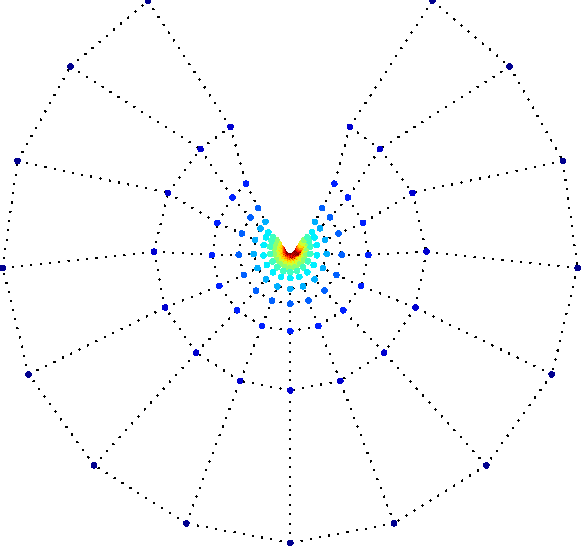
\includegraphics[width = .4\columnwidth]{/Users/fhuszar/Dropbox/thesis/matlab/manifold/figs/Normal_kernel_1.pdf} & $\ell\rightarrow 0$& 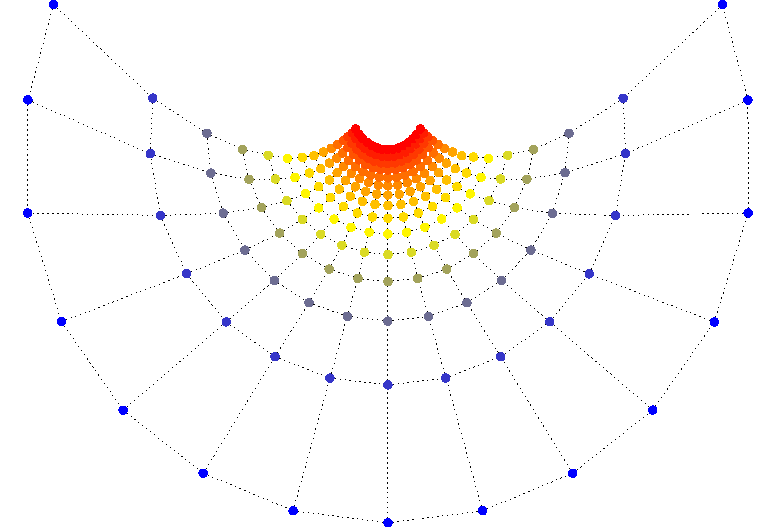
\includegraphics[width = .4\columnwidth]{/Users/fhuszar/Dropbox/thesis/matlab/manifold/figs/Normal_kernel_2.pdf} \\
	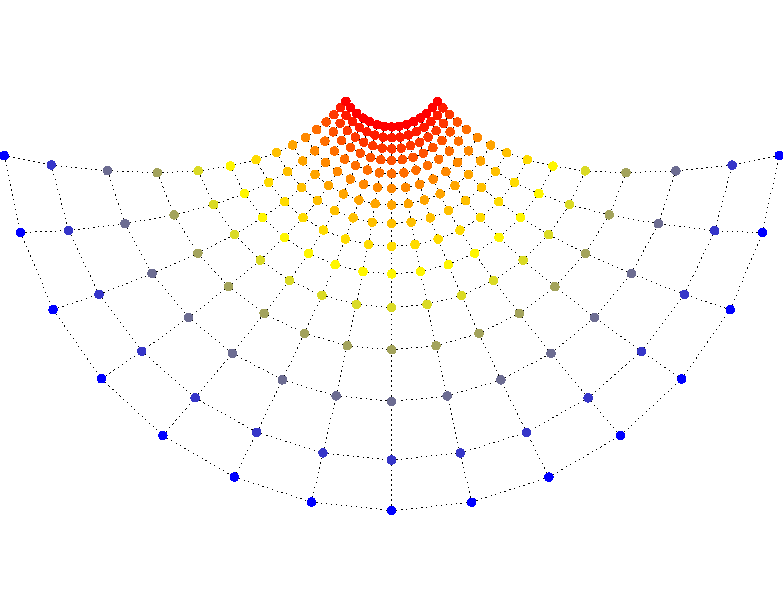
\includegraphics[width = .4\columnwidth]{/Users/fhuszar/Dropbox/thesis/matlab/manifold/figs/Normal_kernel_3.pdf} & $\ell=0.5$ & 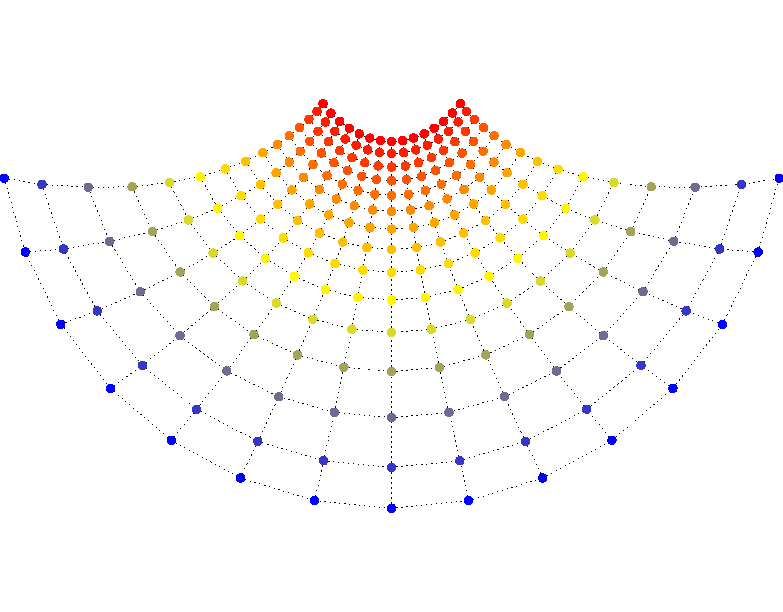
\includegraphics[width = .4\columnwidth]{/Users/fhuszar/Dropbox/thesis/matlab/manifold/figs/Normal_kernel_4.pdf} \\
	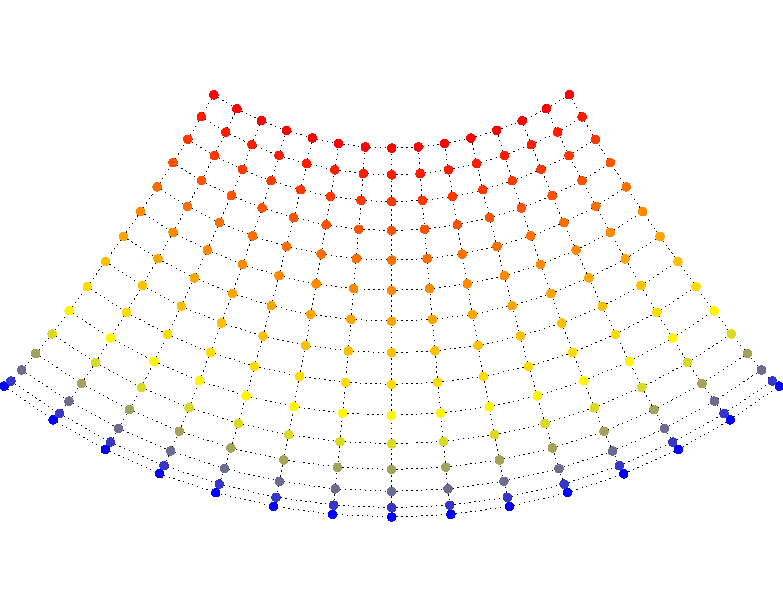
\includegraphics[width = .4\columnwidth]{/Users/fhuszar/Dropbox/thesis/matlab/manifold/figs/Normal_kernel_5.pdf} & $\ell=2$ &  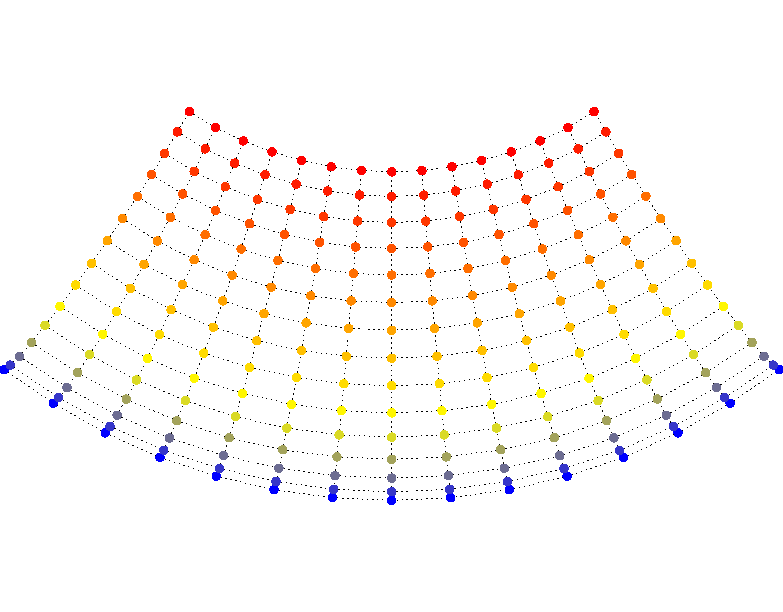
\includegraphics[width = .4\columnwidth]{/Users/fhuszar/Dropbox/thesis/matlab/manifold/figs/Normal_kernel_6.pdf} \\
	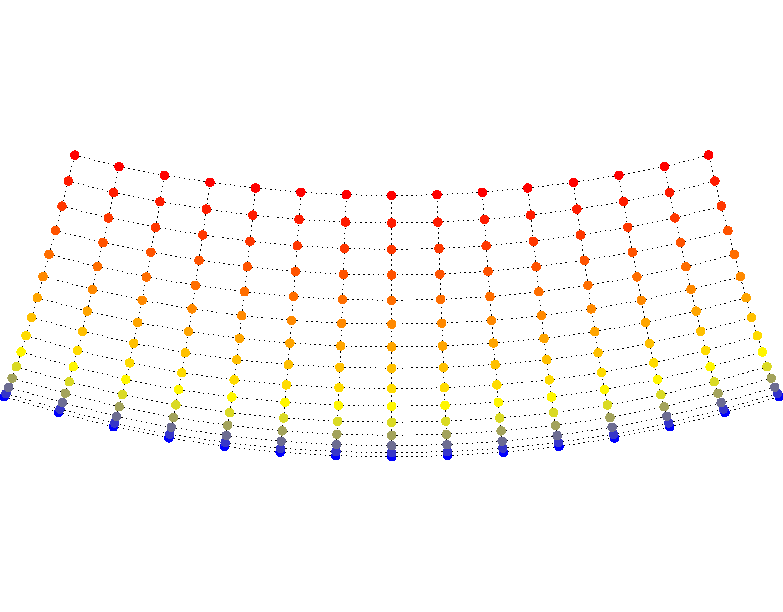
\includegraphics[width = .4\columnwidth]{/Users/fhuszar/Dropbox/thesis/matlab/manifold/figs/Normal_kernel_7.pdf} & $\ell=5$ &  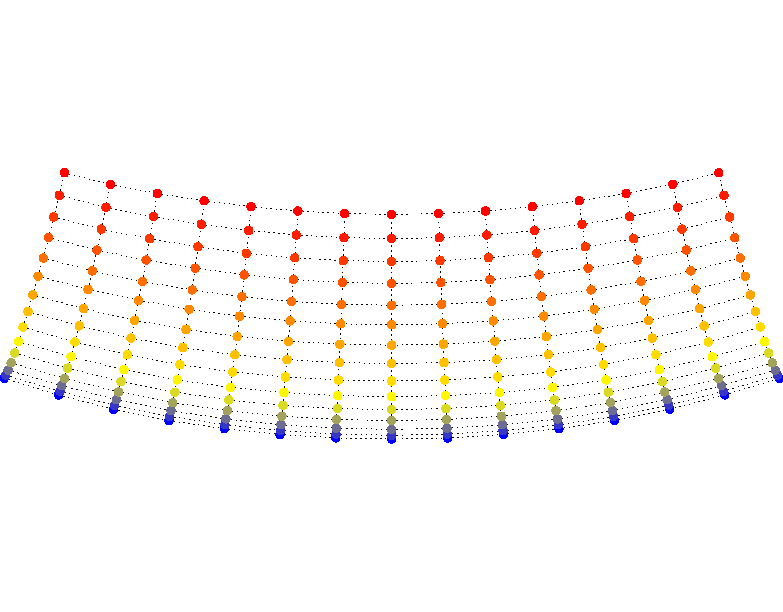
\includegraphics[width = .4\columnwidth]{/Users/fhuszar/Dropbox/thesis/matlab/manifold/figs/Normal_kernel_8.pdf} \\
	\end{tabular}
	\end{center}
	\caption{Maps of the statistical manifold induced by the (quadratic) kernel score and the spherical kernel score over Gaussian distributions for different setting of the kernel bandwidth parameter. The two panels in the top row $\ell\rightarrow 0$ correspond to the limiting cases of the Brier score and the spherical score. It can be seen that as the bandwidth increases, both scores shift their sensitivity to distributions with higher variance (red). For equal bandwidth, the spherical kernel score is more sensitive to distributions with larger standard deviation.}
\end{figure}

The main purpose of this section is to visualise differences between the geometries induced by various divergence measures over the same set of distributions. A particularly interesting divergence that we will use in subsequent chapters is that induced by the (quadratic) kernel scoring rule from (section \ref{sec:kernel_scoring}). The kernel scoring rule itself is very flexible, and its properties are dictated by the choice of kernel function.

For several well-known kernels the divergence between univariate Gaussians can be computed in closed form.\citep{tailoring_density} For the squared exponential kernel $k_{\ell}(x,x')=\nicefrac{1}{\ell}\exp(-\frac{(x-x')^2}{\ell^2})$ the divergence is given by the following formula:

\begin{equation}
	\divergence{k_{\ell}}{\Normal_{\mu_1,\sigma_1}}{\Normal_{\mu_2,\sigma_2}} = \frac{1}{\sqrt{\ell^2+2\sigma_1^2}} + \frac{1}{\sqrt{\ell^2+2\sigma_2^2}} - \frac{2}{\sqrt{\ell^2+\sigma_1^2 + \sigma_2^2}}\exp\left(-\frac{(\mu_1 - \mu_2)^2}{2(\ell^2 + \sigma_1^2 + \sigma_2^2)}\right)
\end{equation}

The above formula can be derived from the following general expression for the inner product between mean embeddings:

\begin{align}
	\scalar{\mu_{\Normal(\mu_1,\sigma_1)}}{\mu_{\Normal(\mu_2,\sigma_2)}}_{k_{\ell}} &= \expect{x\sim \Normal(\mu_1,\sigma_1)}\expect{x' \sim \Normal(\mu_1,\sigma_1)} k_{\ell}(x,x')\\
	&= \frac{1}{\sqrt{\ell^2 + \sigma_1^2 + \sigma_2^2}}\exp\left(-\frac{(\mu_1 - \mu_2)^2}{2(\ell^2 + \sigma_1^2 + \sigma_2^2)}\right)
\end{align} 

The first fact one may observe is that unlike the KL divergence, the kernel divergence is bounded from above by $\nicefrac{2}{\ell}$. This upper bound is approached when computing divergence between two infinitesimally narrow Gaussians $\sigma_1,\sigma_2\approx 0$ that are far apart $\vert \mu_1 - \mu_2 \vert > 0$. The divergence is also bounded from below by $0$ and it is $0$ exactly when the two distributions are identical, confirming that this kernel function gives rise to a strictly proper scoring rule.

The Brier score is a special case of this divergence as the lengthscale of the kernel $\ell$ decreases to $0$. In that case we obtain the following expression:

\begin{equation}
	\divergence{Brier}{\Normal_{\mu_1,\sigma_1}}{\Normal_{\mu_2,\sigma_2}} = \frac{1}{\sqrt{2\sigma_1^2}} + \frac{1}{\sqrt{2\sigma_2^2}} - \frac{2}{\sqrt{\sigma_1^2 + \sigma_2^2}}\exp\left(-\frac{(\mu_1 - \mu_2)^2}{2(\sigma_1^2 + \sigma_2^2)}\right)
\end{equation}

We can immediately see that unlike the kernel score with a positive lengthscale, the Brier score is not bounded from above. It diverges for very small values of the variances $\sigma_1$ and $\sigma_2$. It is still non-negative and strictly proper.

To illustrate the differences between the various divergences between Gaussian distributions, we first applied the ISOMAP embedding technique to the one-dimensional manifold of zero-mean Gaussians, whose sole free parameter is the standard deviation. I chose a logarithmically spaced grid of standard deviation values, then used the ISOMAP algorithm to embed the distributions on the real line. The logarithmic spacing is useful as the KL divergence now depends only on the difference in the logarithm of variances, therefore when these distributions are embedded according to the KL divergence, we expect to get a uniform, linearly spaced grid.

Figure \ref{fig:fig:Normal_varonly_comparison} compares the statistical manifold induced by the KL and Brier divergences, as well as by the kernel divergence with different choices of the kernel bandwidth parameter $\ell$. As expected, when the KL divergence is used the numerical algorithm spreads the distributions uniformly on the real line. We can see that compared to the KL divergence, the Brier divergence is more sensitive to differences between narrow distributions, whose standard deviation is small. In case of the kernel score, with increasing kernel brandwith the focus shifts from narrow distributions towards distributions with larger variance. In the range mapped in this figure ($0.05 \leq \sigma \leq 1$) the kernel bandwidth $\ell=0.1$ mimics the behaviour of the KL divergence the best.

For these distributions the KL divergence is scale-free: the divergence between two zero-mean Gaussians with variance $\sigma_1=0.05$ and $\sigma_2 = 0.1$ is the same as the divergence between $\sigma_1=0.5$ and $\sigma_2 = 1$. The kernel score on the other hand has a characteristic brandwith, and is therefore not scale free: when the brandwith is chosen to be $\ell=1$, the largest shown in Figure $\ref{fig:Normals_kernel_comparison}$, the distance between $\sigma_1=0.05$ and $\sigma_2 = 0.1$ is only about one tenth of the distance between $\sigma_1=0.5$ and $\sigma_2 = 1$.

In Figure \ref{fig:Normals_varonly_magnification} I plotted the local distances on the various manifolds relative to distances induced by the logarithmic score. Higher values on the plot indicate a region where local distances are magnified in comparison to the KL divergence, which can be interpreted as a region in which the particular scoring rule is more sensitive to small differences. Observe how changing the kernel bandwidth shifts the most sensitive region of the kernel scoring rule.

These figures highlight how the choice of the kernel allows us to fine-tune properties of the divergences and the corresponding manifold. We can use this flexibility to tailor the divergence to our application \citep{tailoring}. However, as discussed in chapter \ref{sec:scoring_rules} this flexibility also poses a challenge in applications where there is no principled way of choosing kernel hyperparameters.

\subsection{Gamma distributions}

We can look at the geometry Shannon's entropy induces within another two-parameter family of continuous distributions, Gamma distributions. Gamma distributions are strictly positive, their probability density function of Gamma distributions is as follows:

\begin{equation}
(x) = \beta^{\alpha}\frac{1}{\Gamma(\alpha)} x^{\alpha-1} \exp(-\beta x)
\end{equation}

where $\alpha,\beta > 0$ are called shape and rate parameters respectively. Special cases of Gamma distributions are exponential distributions when $\alpha=1$.

The KL divergence between Gamma distributions can be computed in closed form and is given by the following formula:

\begin{equation}
	\KL{\Gamma_{\alpha_1,\beta_1}}{\Gamma_{\alpha_2,\beta_2}} = \left(\alpha_1 - \alpha_2\right)\psi\left(\alpha_1\right) - \log\frac{\Gamma(\alpha_1)}{\Gamma(\alpha_2)} + \alpha_1\log\frac{\beta_1}{\beta_2} + \alpha_1\frac{\beta_2 - \beta_1}{\beta_1} \label{eqn:KL_Gamma}
\end{equation}

\begin{figure} % Gamma distribution - Shannon information statistical manifold
	\begin{center}
	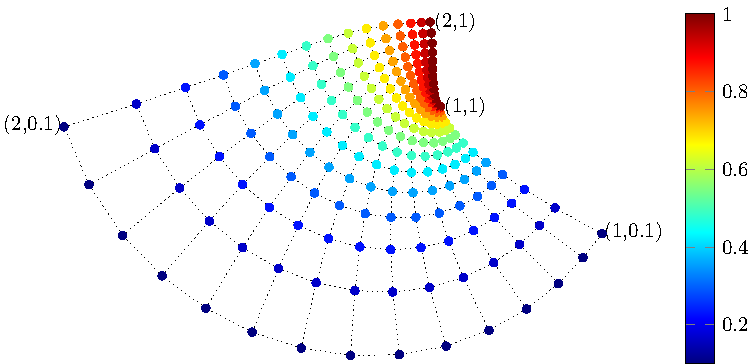
\includegraphics{/Users/fhuszar/Dropbox/thesis/matlab/manifold/figs/Gamma_meanvar.pdf}
	\end{center}
	\caption{Map of Gamma distributions on the statistical manifold induced by the logarithmic score and KL divergence. To be comparable to the manifold of Normal distributions in Figure \ref{fig:Normal_meanvar}, the distributions are parametrised by their mean and standard deviation. Distributions are chosen from a uniform grid in this non-standard parameter-space, with their mean ranging between $1$ and $2$, and standard deviation between $0.1$ and $1$. For large values of variance \emph{(yellow and red)} the manifold is asymmetric and dissimilar to that of Normal distributions. However, as variance decreases \emph{(blue)}, by the central limit theorem Gamma distributions approach Gaussians of the same mean and variance, thus the manifold conforms to the fan-like shape that is characteristic of Gaussian distributions.}
\end{figure}

Figure \ref{fig:Gamma_embedding} shows the manifold of Gamma distributions for parameters $a \leq \alpha \leq b, c\leq \beta \leq d$. As we can see this manifold is less symmetric than that of the Gaussians.

For large values of $\alpha$ the standard deviation of the distribution shrinks, and by the central limit theorem, the distribution converges to a Gaussian. We can illustrate this convergence in the manifold structure. For this we first reparametrise the Gamma distribution in terms of its mean and standard deviation. The mean and standard deviation of a Gamma distribution with parameters $\alpha$ and $\beta$ are given by the following formulae:

\begin{align}
	\mu &= \frac{\alpha}{\beta}\\
	\sigma^2 &= \frac{\alpha}{\beta^2}
\end{align}

Solving for $\alpha$ and $\beta$ in these equations we get

\begin{align}
	\alpha &= \frac{\mu^2}{\sigma^2}\\
	\beta &= \frac{\mu}{\sigma^2}
\end{align}

Plugging these into Eqn.\ \eqref{eqn:KL_Gamma} we can now map Gamma distributions with particular mean and variance. Figure 1 compares Normal and Gamma distributions with mean $\mu\in[0.5,1.5]$ and standard deviation $\sigma\in[0.1,1]$. We can observe that as the variance increases, the manifold of Gamma distributions shows a fan-like structure very similarly that of Normal distributions. However, for larger variance, the distributions look less Gaussian, and the manifold becomes more asymmetric. The effect of the central limit theorem would perhaps be even more prominent for smaller values of $\sigma$, but for those cases that case Eqn.\ \eqref{eqn:KL_Gamma} becomes numerically imprecise, as it relies on look-up-table implementation of the Gamma ($\Gamma$) and bigamma ($\psi$) functions.

% \subsection{Reactor example}

% Not all scoring rules give rise to smooth manifolds. As an extreme example, consider the following decision problem:

% You are uncertain about the temperature of the reactor in a power plant. If the temperature is too high, above a critical temperature $T_{crit}$, the reactor may melt down causing you a loss of \$10 billion. You may choose to shut down the reactor, which costs you \$1 million of lost revenue, irrespective of whether the reactor was indeed overheated or not. You make a probabilistic forecast about the reactor's temperature, and want to make a decision based on that.

% This decision rule segments probabilistic forecasts into only two subsets: those which would result in a ``shut down'' decision, and those that result in a ``keep on going''. 

% \begin{equation}
%   \divergence{reactor}{p}{q} = \left\{
%   \begin{array}{cc} 
%       \begin{array}{cc}
%         0        & p(\{t\geq T_{crit}\}) \geq \ell \mbox{ and } q(\{t\geq T_{crit}\}) \geq \ell\\
%         \ell_1 & p(\{t\geq T_{crit}\})  \geq \ell \mbox{ and } q(\{t\geq T_{crit}\}) \leq \ell\\
%         \ell_2 & p(\{t\geq T_{crit}\})  \leq \ell \mbox{ and } q(\{t\geq T_{crit}\}) \geq \ell
%       \end{array}
%   \end{array}
%   \right.
% \end{equation}

% This divergence therefore does not give rise to a smooth manifold. Figure \ref{fig two_points} shows a map of Gaussian distributions with respect to the KL divergence. The way $\divergence{reactor}{\cdot}{\cdot}$ segments distributions into ``shut down'' or ``keep on going'' types is also shown. We can make the KL divergence more sensitive to the decision problem at hand by considering a convex combination between $\KL{\cdot}{\cdot}$ and $\divergence{reactor}{\cdot}{\cdot}$.

